%
% loesung.tex -- Beispiel-File für die Beschreibung der Loesung
%
% (c) 2020 Prof Dr Andreas Müller, Hochschule Rapperswil
%
\section{Anwendungen
\label{pade:section:Anwendungen}}
\rhead{Anwendungen}

In diesem Abschnitt werden ein paar Anwendungsmöglichkeiten der Padé-Approximation gezeigt.
Wie in der Signalverarbeitung in der Elektrotechnik üblich, werden des öfteren mathematische Probleme im Frequenzbereich gelöst, da dies oft einfacher ist. 
Die Transformation in das geeignete Spektrum kann bei kontinuierlichen Signalen mit der Laplace-Transformation und bei diskreten Signalen mit der Z-Transformation erreicht werden.
Unter dem Begriff Übertragungsfunktion, versteht man das Verhältnis von Ausgangssignal / Eingangssignal.
Die Abhängigkeit der verschiedenen Zustandsräumen wird folgend mit dem Beispiel der Übertragungsfunktion $h(t)$ dargestellt.
\begin{center}
	\tikzset{>=latex}
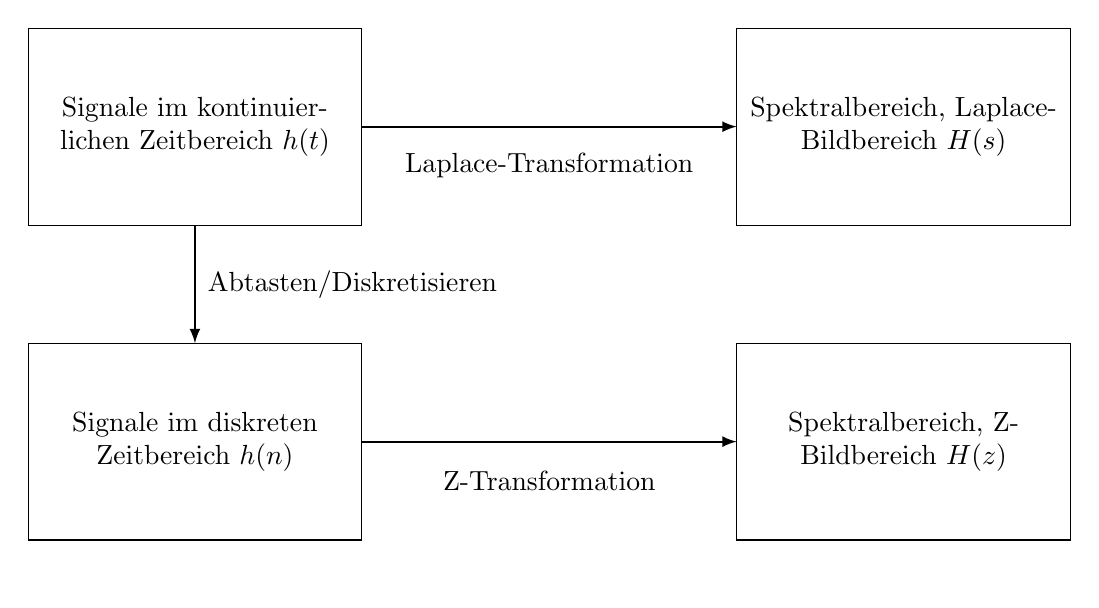
\begin{tikzpicture}
\node[draw,text width=4cm,minimum height=2.5cm,align=center] at (0,0) {Signale im kontinuierlichen Zeitbereich $h(t)$};
\node[draw,text width=4cm,minimum height=2.5cm,align=center] at (0,-4) {Signale im diskreten Zeitbereich $h(n)$};
\node[draw,text width=4cm,minimum height=2.5cm,align=center] at (9,0) {Spektralbereich, Laplace-Bildbereich $H(s)$};
\node[draw,text width=4cm,minimum height=2.5cm,align=center] at (9,-4) {Spektralbereich, Z-Bildbereich $H(z)$};

\draw[thick,->] (2.12,0)--(6.88,0);
\draw[thick,->] (2.12,-4)--(6.88,-4);
\draw[thick,->] (0,-1.25)--(0,-2.75);

\node[text width=4cm,minimum height=2.5cm,align=center] at (4.5,-0.5) {Laplace-Transformation};
\node[text width=4cm,minimum height=2.5cm,align=center] at (2,-2) {Abtasten/Diskretisieren};
\node[text width=4cm,minimum height=2.5cm,align=center] at (4.5,-4.5) {Z-Transformation};
\end{tikzpicture}
\end{center}
Dabei gelten $s= \sigma+ j\omega$ und $z = A e^{j\omega} =\sigma+ j\omega$.
Der jeweilige Spektralbereich wird auch oft Bildbereich genannt.

\subsection{Totzeit Approximation
\label{pade:subsection:totzeit}}

Bei der Totzeit spricht man von einer Verzögerung im Zeitbereich, welche zum Beispiel in einem digitalen Regelkreis vorkommen kann.
Lineare zeitinvariante (LZI)-Systeme oder besser bekannt unter dem englischen Begriff linear time-invariant (LTI) system, sind unabhängig von zeitlichen Verschiebungen. 
Die Eingangs- Ausgangsbeziehung von LTI-Systemen, ist durch die zeit-diskrete Faltung der Impulsantwort des Systems mit dem Eingangssignal gegeben. 
LTI-Systeme können in zwei Typen  eingeteilt werden.
Der erste Typ ist die finite impulse response (FIR) mit endlicher Impulsantwort.
Typ zwei hat eine unendlich lange Impulsantwort, genannt die infinite impulse response (IIR).
Diese zwei Typen unterteilen Impulsantworten anhand der Eigenschaft ob sie eine endliche oder unendliche Dauer hat. 
Wer sich mit LTI Systemen auseinander gesetzt hat, weiss, dass eine Totzeit $T$ im Frequenzbereich durch eine Exponentialfunktion
\begin{equation*}
H(s) = e^{-sT}
\end{equation*}
ausgedrückt wird.

Verschiedene Methoden wie z.B. die Wurzelortskurven können nicht mit einer Totzeit umgehen, sondern nur mit Übertragungsfunktionen, welche normalerweise als gebrochen rationale Funktionen vorliegen.
Die Übertragungsfunktion besteht aus einem Nenner- und Zählerpolynom welches der Form
\begin{equation*}
H(s)=\frac{P(s)}{Q(s)}
\end{equation*}
entspricht.

Beim Design von Filtern, Reglern oder anderen Frequenzabhängigen Netzwerken, verwendet man die Laplace- oder Z-Transformierte der Übertragungsfunktion, um die Eigenschaften des zu entwerfenden Netzwerkes zu synthetisieren / analysieren.
Dazu benötigt man nun die Übertragungsfunktion in Form von gebrochenen Polynomen, mit welchen man zum Beispiel die Pol- und Nullstellen des Netzwerkes erkennt.
Mit diesen Pol- und Nullstellen können aussagen über den Betrags- und Phasenverlauf des Frequenzgangs, Impuls- und Sprungantwort, Stabilität eines Systems und weitere Eigenschaften gemacht werden.
Mit diesen Informationen kann entschieden werden, welche Parameter geändert werden müssen um die gewünschten Eigenschaften zu erhalten.
 
Diese Netzwerke werden oft mit passiven Bauelementen wie Widerständen, Induktivitäten und Kapazitäten und einem Operationsverstärker realisiert.
Ein PID-Glied kann so zum Beispiel in vereinfachter Form wie folgt Konstruiert werden.
\begin{center}
	\tikzset{>=latex}
\begin{tikzpicture}
\node[text width=4cm,minimum height=2.5cm,align=center] at (0,0.25) {Input};
\node[text width=4cm,minimum height=2.5cm,align=center] at (8.5,-0.25) {Output};
\node at (2,0.5) {$R_1$};
\node at (5.5,2) {$R_2$};

\node at (2,-1.25) {$C_1$};
\node at (4.1,1.25) {$C_2$};

\draw[thick] (0,0)--(1,0)--(1,0.5)--(1,-0.5);
\draw[thick] (1,-0.5)--(1.9,-0.5)--(1.9,0)--(1.9,-1);
\draw[thick] (2.1,-1)--(2.1,0)--(2.1, -0.5)--(3,-0.5)--(3,0.5)--(2.5,0.5)--(3,0.5)--(3,0)--(3.5,0)--(3.5,2)--(4,2)--(4,1.5)--(4,2.5);
\draw[thick](4.2,2.5)--(4.2,1.5)--(4.2,2)--(5,2);
\draw[thick] (1,0.5)--(1.5,0.5);
\draw[thick] (6,2)--(7.5,2)--(7.5,-0.5)--(4+2.59808,-0.5)--(9,-0.5);

\draw[draw=black,thick] (1.5,0.25) rectangle ++(1,0.5);
\draw[draw=black,thick] (5,1.75) rectangle ++(1,0.5);

\draw[thick] (3.5,0)--(4,0)--(4,1)--(4+2.59808,-0.5)--(4,-2)--(4,1);
\draw[thick] (4,-1)--(3,-1)--(3,-3)--(2.5,-3)--(3.5,-3);
\draw[thick] (4.2,-1)--(4.4,-1);
\draw[thick] (4.3,-0.9)--(4.3,-1.1);
\draw[thick] (4.2,0)--(4.4,0);
\end{tikzpicture}
\end{center}
Zu diesem Beispiel können nun die dazugehörigen Eingangs- und Ausgangsimpedanzen $Z_0$ und $Z_1$ berechnet werden.
\begin{equation*}
Z_{0}(s)
=
\frac{1+s C_{2} R_{2}}{s C_{2}}
\end{equation*}
\begin{equation*}
Z_{1}(s)
=
\frac{R_{1}}{1+s C_{1} R_{1}}
\end{equation*}
Für die Übertragungsfunktion erhält man damit
\begin{equation*}
H(s)
=
\frac{Z_{0}(s)}{Z_{1}(s)}
=
\frac{1-C_2 R_2 C_1 R_1+ s C_2 R_2 +s C_1 R_1 }{s C_2 R_2}.
\end{equation*}
Die zwei Polstellen befinden sich somit bei $s=0$ was einem DC entsprechen würde.
Die Nullstellen befinden sich bei
\begin{equation*}
s
=
\frac{C_1 R_1 C_2 R_2 -1}{C_1 R_1 + C_2 R_2},
\end{equation*}
abhängig von den Komponenten.
Die Erkenntnisse kann man nun für die Dimensionierung der Bauteile oder für welche Anwendungen dieses PID-Glied nicht geeignet ist, verwenden.

Leider kann mit einem passiven Bauteil keine Exponentialfunktion im Frequenzbereich nachgebaut werden und somit auch keine Totzeit.
In der Praxis wird deshalb die Totzeit oft mit digitalen Bausteinen realisiert, da man digital einfach die Werte speichern kann und zur gewünschten Zeit wieder ausgeben.
Mit $e^{-sT}$ in einem analogen System haben wir jedoch keine brauchbaren Pol- Nullstellen welche mit passiven Bauteilen nachgebaut werden können.  
Dies kann jedoch gefordert sein wenn man eine zeit-kontinuierliche Analyse macht oder einfach keine Digitalbausteine in seiner Schaltung verwenden will.
Eine Lösung dafür könnte nun sein, $e^{-sT}$ zu approximieren und die Approximation für weitere Rechnungen zu verwenden.

Die Padé-Approximation der Exponentialfunktion ist glücklicherweise schon bekannt und kann mit den Formeln \eqref{pade:expP} und \eqref{pade:expQ} für eine beliebig hohe Ordnung ermittelt werden.
Die Qualität dieser Approximation wird ersichtlich, wenn die Padé-Approximanten in einer logarithmischen Skala mit der originalen Funktion vergleichen.
In der Grafik \ref{pade:totzeitexp} zeigt sich, dass die Padé-Approximation mit steigendem Grad bessere Resultate liefert und sich der Exponentialfunktion mehr und mehr annähert.

\begin{figure}[!h]
	\centering
	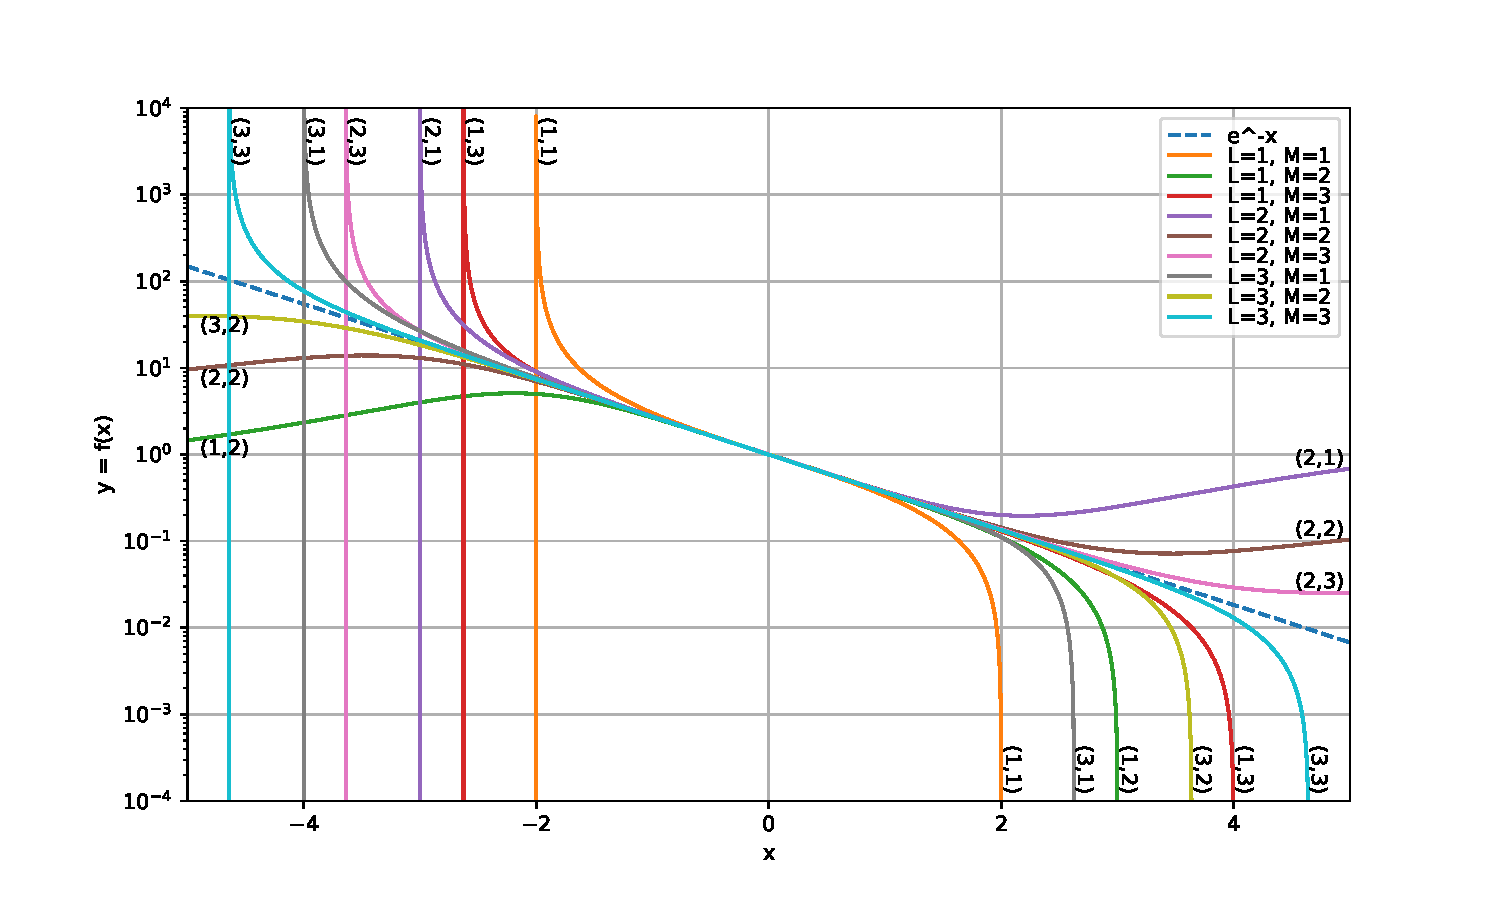
\includegraphics[width=1\linewidth]{./papers/pade/python/bilder/totzeit.pdf}
	\caption{Plot der Padé-Approximanten der Exponentialfunktion im Vergleich zu der Originalfunktion in einer logarithmischen Skala vergleichend mit der Taylor-Reihe sechster Ordnung der Exponentialfunktion.\label{pade:totzeitexp}}
\end{figure}

Im Beispiel \ref{pade:totzeitexp} mit der Exponentialfunktion erweisen sich die Padé-Approximanten des selben Grades im Nenner und Zähler als die genauesten Approximationen.
Es wird dabei mit steigendem Grad der Approximation eine stetige Verbesserung erzielt.
Zum Vergleich ist noch die Taylor-Reihe von $e^{-x}$ der sechsten Ordnung in der Grafik \ref{pade:totzeitexp} dargestellt. 
Diese ist im negativen Bereich der Funktionsachse deutlich schlechter als die Padé-Approximanten, jedoch verhält sie sich im positiven Bereich besser.


Transferieren wir nun diese gebrochenen Polynome, welche sich noch im Frequenzbereich befinden zurück in den Zeitbereich, erhalten wir die in der Grafik \ref{pade:totzeitexp2} dargestellten Kurven.

\begin{figure}[!h]
	\centering
	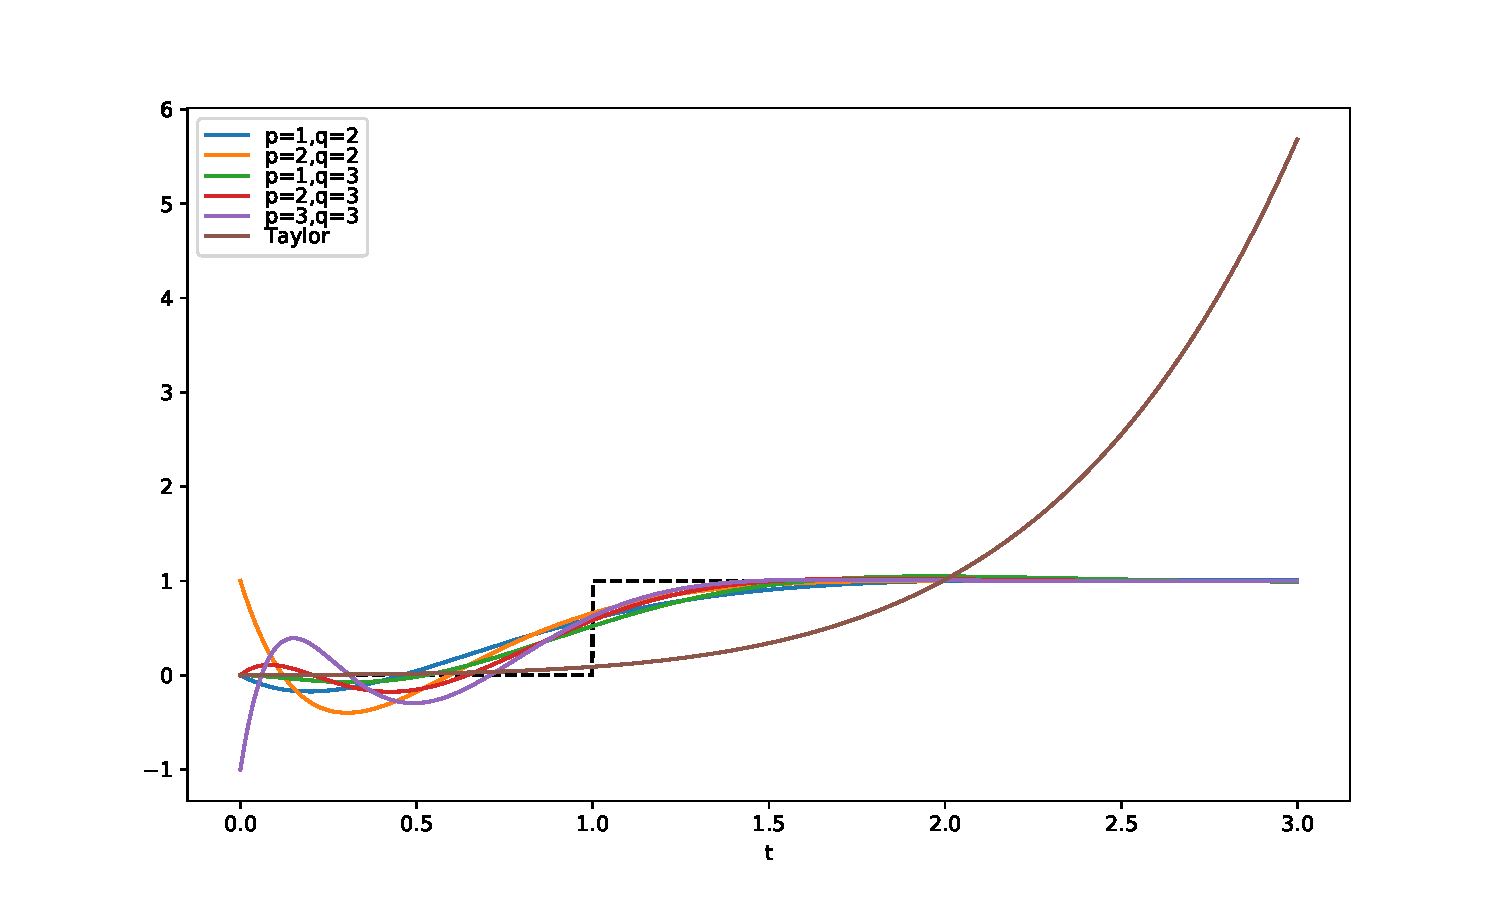
\includegraphics[width=1\linewidth]{./papers/pade/python/bilder/padelow33.pdf}
	\caption{In den Zeitbereich rücktransformierte Padé-Approximanten tieferer Ordnungen\label{pade:totzeitexp2}.}
\end{figure}

Die Polynome der Ordnung $[3/3]$ sind dabei noch weit von einem brauchbaren Ergebnis des gesuchten verzögerten Einheitssprunges entfernt.
Man kann nun die Ordnung der Padé-Approximanten weiter erhöhen bis eine zufriedenstellende Approximation vorliegt.
Dabei muss jedoch aufgepasst werden welche Methode für die Rücktransformation verwendet wird.
Nicht alle Implementationen der Rücktransformation von Übertragungsfunktionen in ein Zustandsraummodell sind numerisch stabil. 
Bei Polynomen grosser Ordnung oder wenn das Nenner- und Zähler- Polynom nicht gleicher Ordnung sind, können bei einer Rücktransformation Fehler auftauchen.
Dies ist jedoch ein anderes Thema, welches den Rahmen dieses Papers sprengen würde.


\begin{figure}[h]
	\centering
	\subfigure[Pole- und Nullstellen in der komplexen Ebene wenn $P=Q$ ist.\label{pade:poles1}]{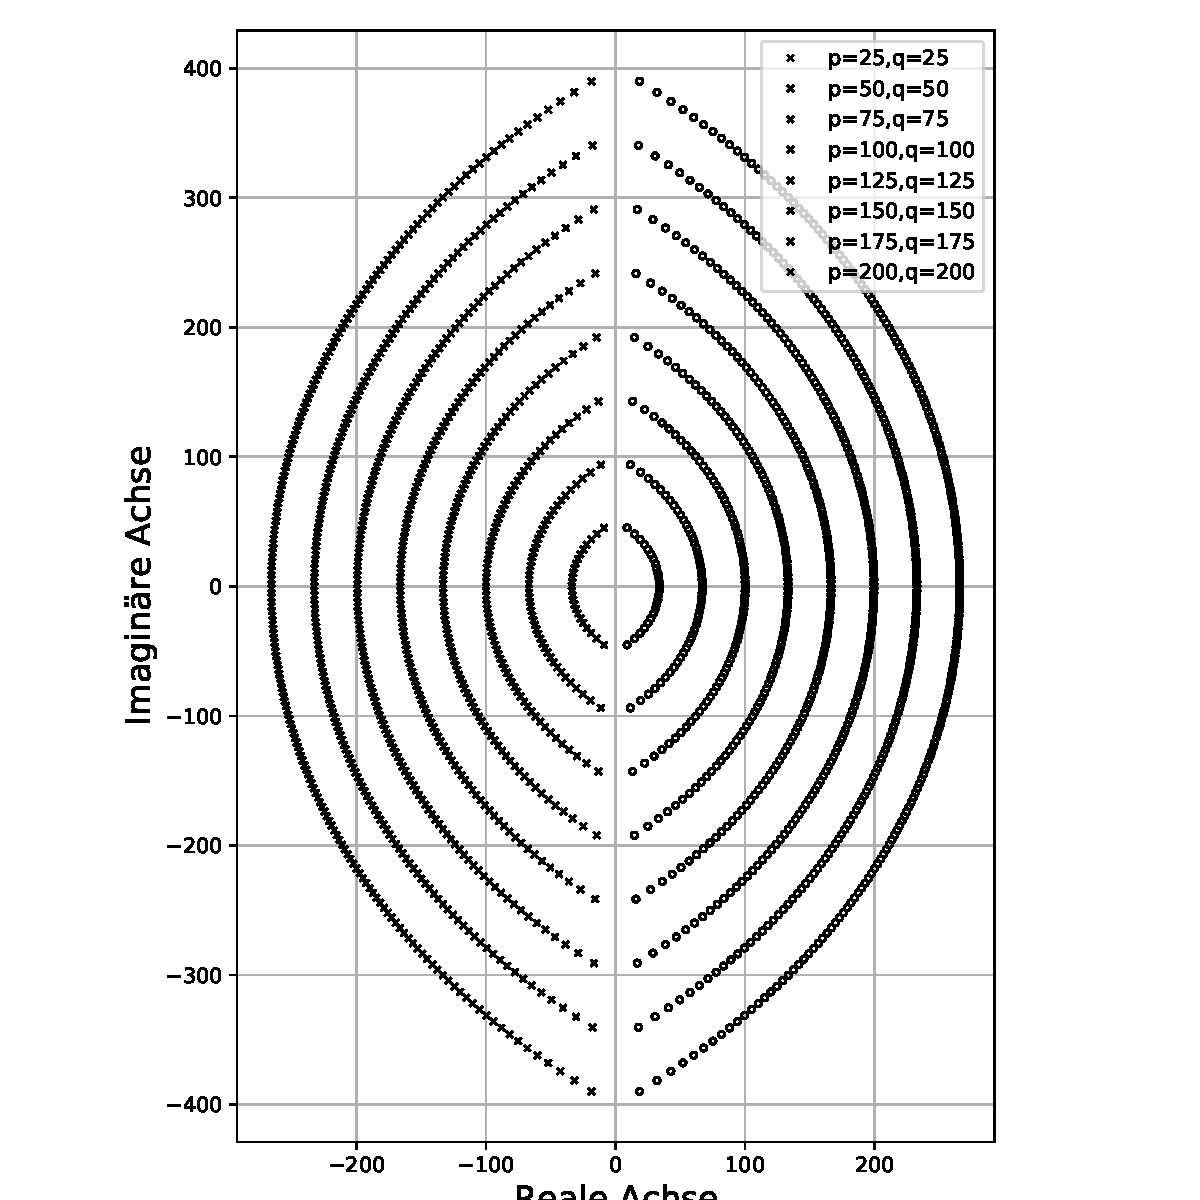
\includegraphics[width=0.40\linewidth]{./papers/pade/python/bilder/poles1.pdf}}
	\subfigure[Pole- und Nullstellen in der komplexen Ebene wenn $P>Q$ ist.\label{pade:poles2}]{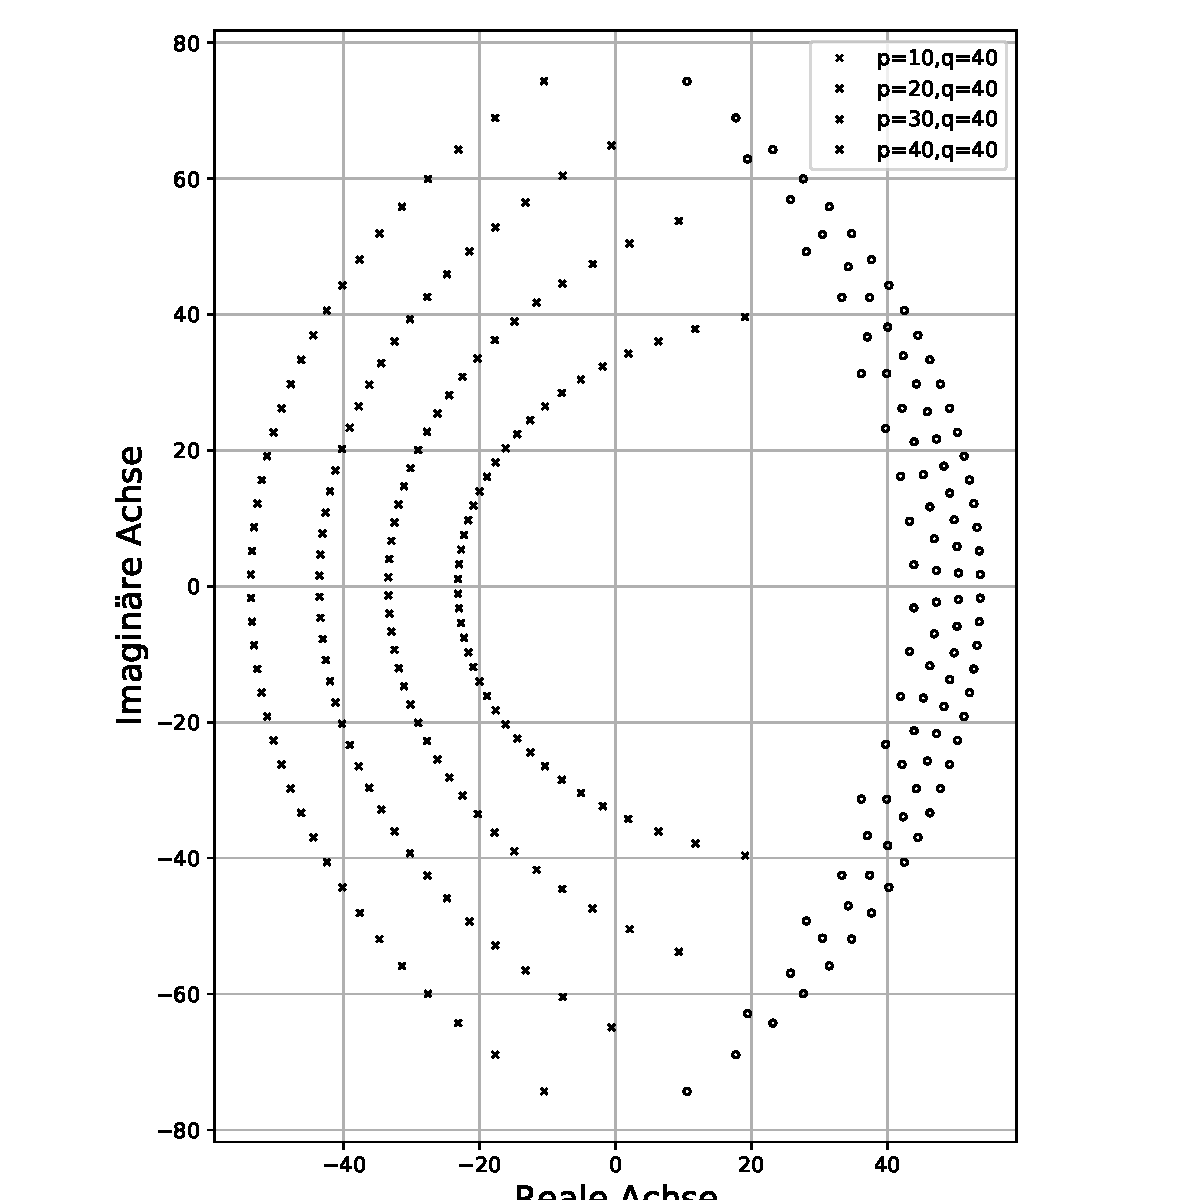
\includegraphics[width=0.40\linewidth]{./papers/pade/python/bilder/poles2.pdf}}
	\subfigure[Pole- und Nullstellen in der komplexen Ebene wenn $P<Q$ ist.\label{pade:poles3}]{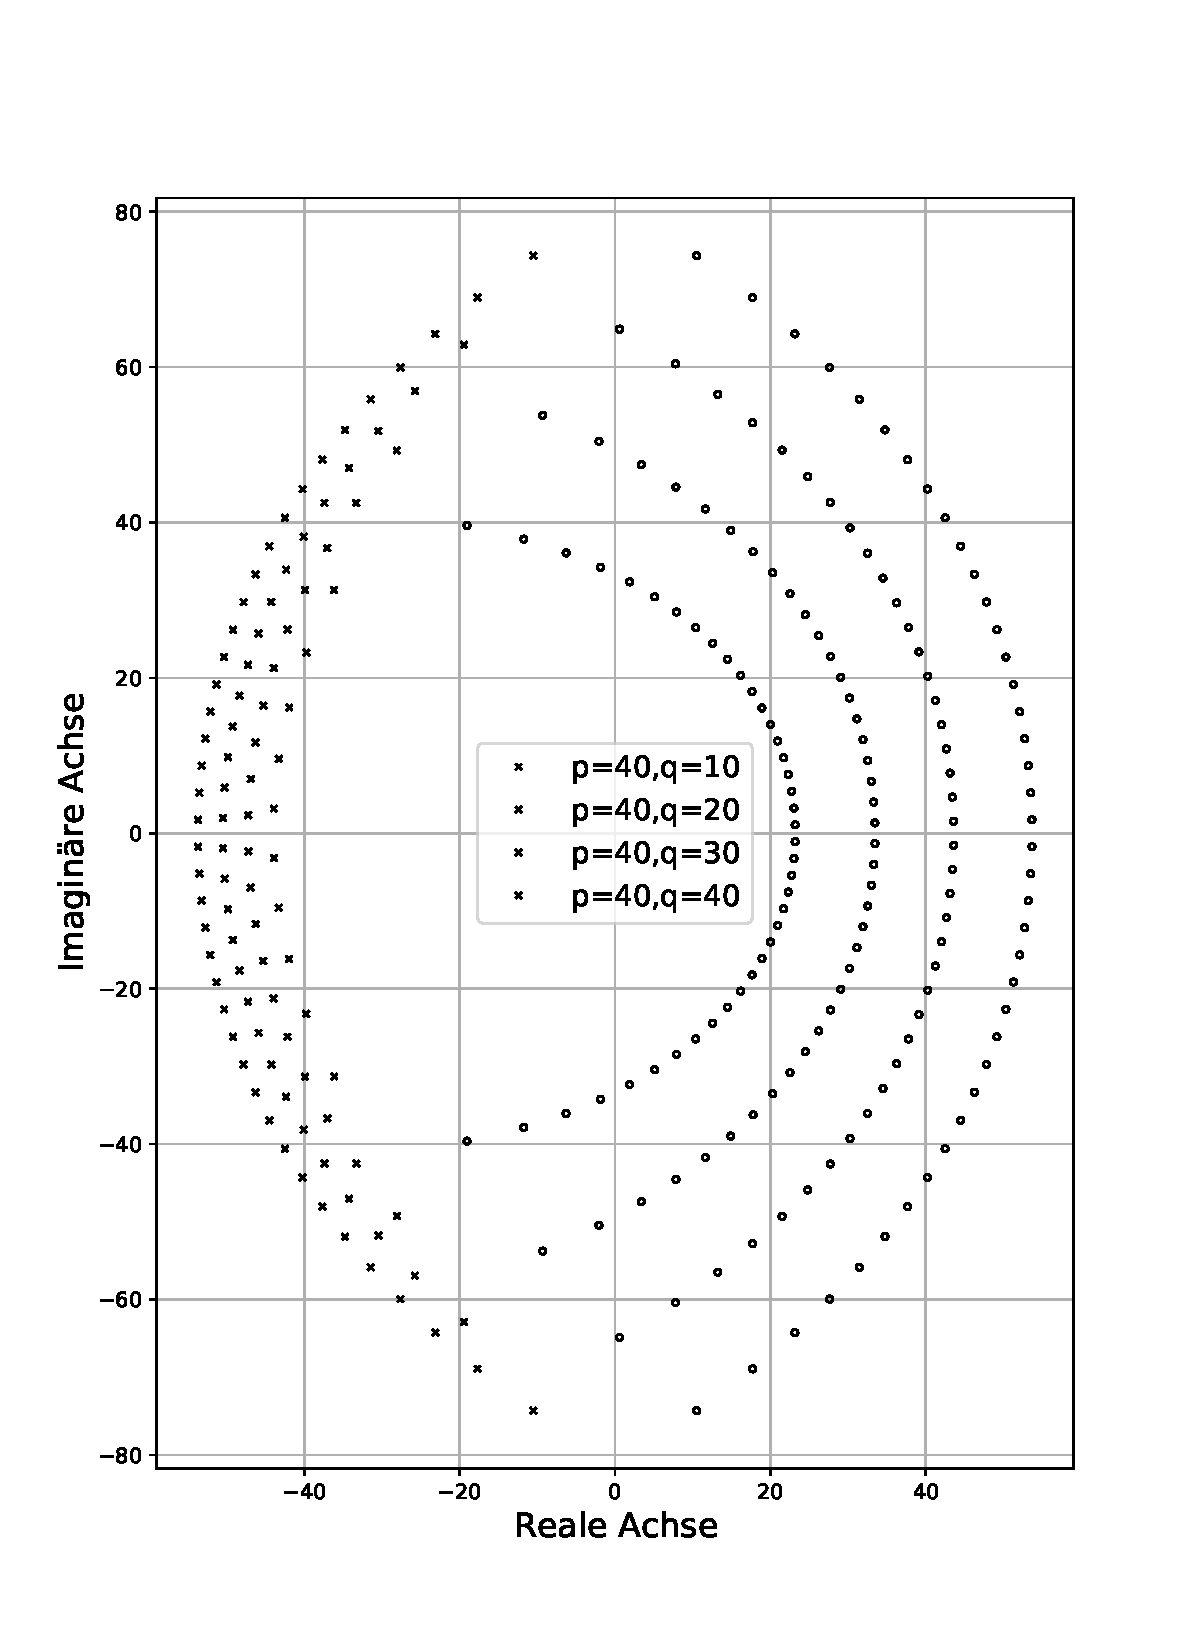
\includegraphics[width=0.40\linewidth]{./papers/pade/python/bilder/poles3.pdf}}
	\caption{Visualisierung der Stabilität der Padé-Polynome bei ungleicher $[L/M]$ Ordnung. \label{pade:prole}}
\end{figure}

In der Grafik \ref{pade:prole} sind nun die Pol- und Nullstellen von höheren Ordnungen dargestellt. 
Auffallend ist die schöne Symmetrie der Pol- und Nullstellen welche bei gleicher Ordnung der Nenner- und Zähler- Polynome um den Nullpunkt verteilt sind.
Diese Symmetrie verschwindet wenn der Grad des Nenner- oder des Zähler- Polynoms grösser gewählt wird.
Dies kann man soweit treiben, bis eine Polstelle in den rechten Bereich der komplexen Halbebenen reicht \ref{pade:poles2},
was ein instabiles System zur Folge hat.
Ein instabiles System beutetet hier, dass der rücktransformierte Einheitssprung eine anwachsende Schwingung ist.
 
\begin{figure}
	\centering
	\subfigure[Rücktransformation der Padé-Approximanten im Zeitbereich geplottet wenn $P=Q$ ist.\label{pade:totzeit1}]{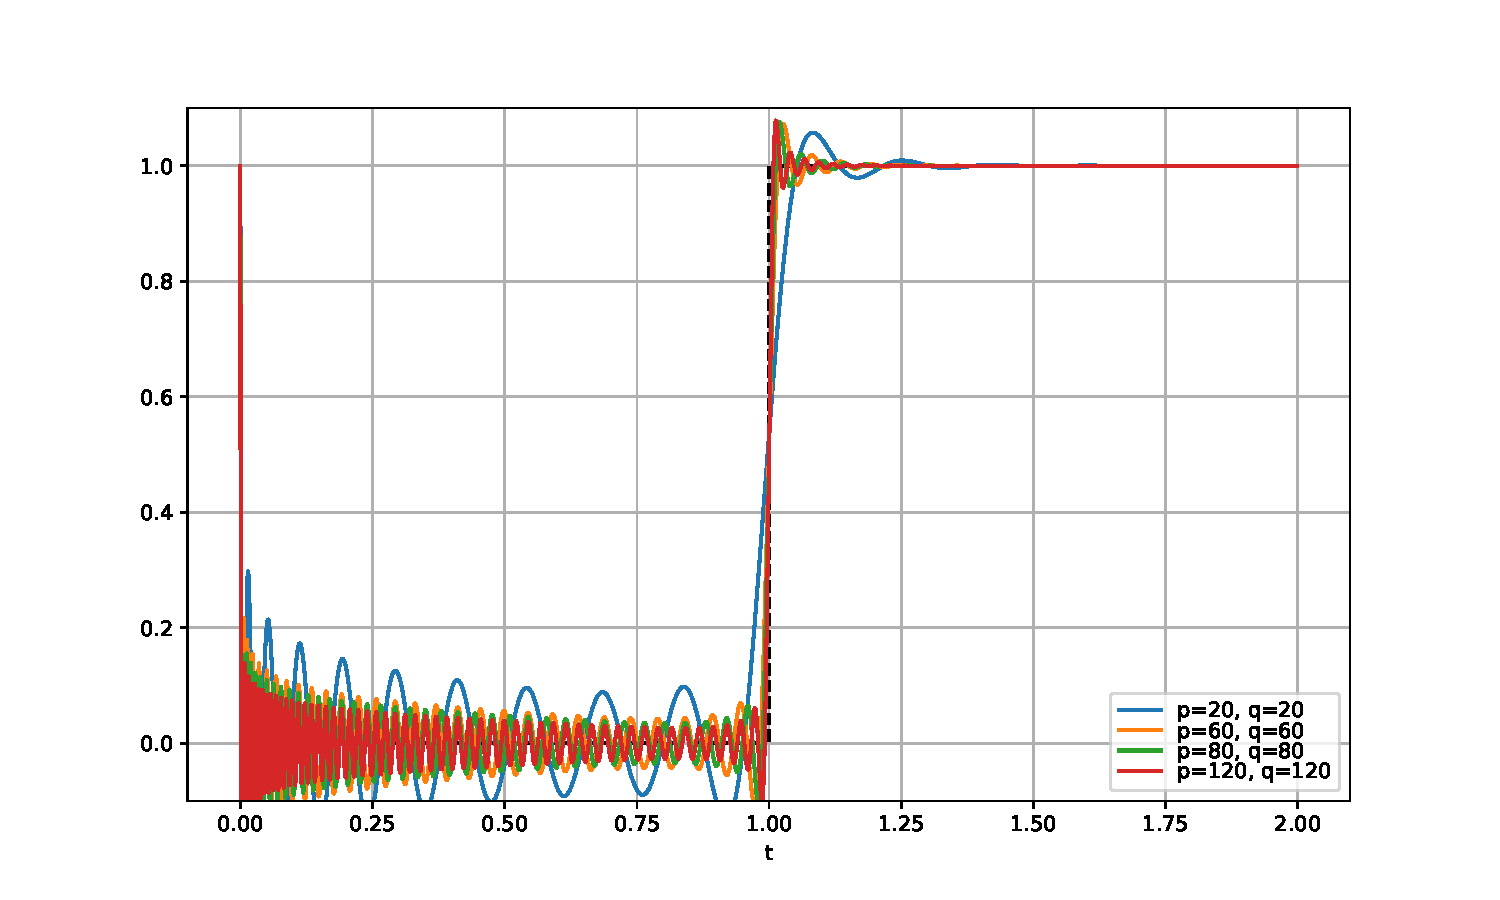
\includegraphics[width=1\linewidth]{./papers/pade/python/bilder/padehigh1.pdf}}
	\subfigure[Rücktransformation der Padé-Approximanten im Zeitbereich geplottet wenn $P=Q-10$ ist.\label{pade:totzeit2}]{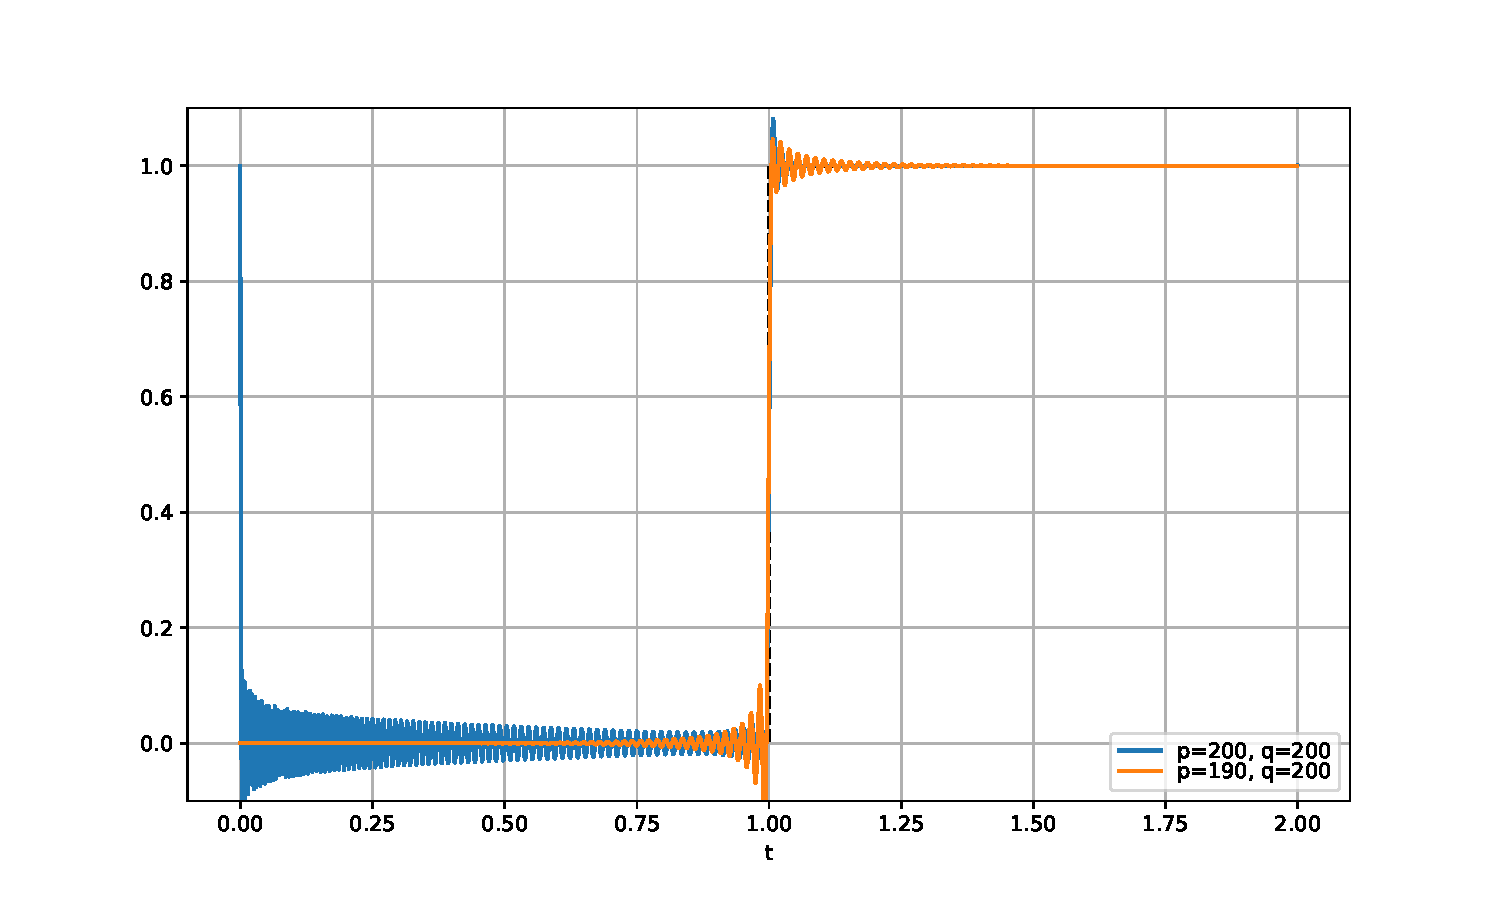
\includegraphics[width=1\linewidth]{./papers/pade/python/bilder/padehigh2.pdf}}
\end{figure}
Verwendet man nun die Approximanten höherer und gleicher Ordnung für die Rücktransformation in Grafik \ref{pade:totzeit1}, erhält man einen immer besser werdenden Einheitssprung mit einem kleinen Überschwinger vor und nach dem Sprung. 
Auffallend ist hier, dass der Padé-Approximant höchster Ordnung zu Beginn den grössten Fehlerpeak hat.
Dieser ist sogar so hoch wie der Einheitssprung selbst.

Um diesen Fehlerpeak zu Beginn ein wenig zu vermindern, können nun die Pole in der komplexen Ebene ein wenig näher zur positiven Halbebene gebracht werden.
Wie schon in  dem Pol- Nullstellendiagramm \ref{pade:poles2} erkennbar, ist das mit einer Differenz von der Ordnung des Zählerpolynoms $p$ und Nennerpolynom $q$ möglich.
Mit einer Differenz von 190 zu 200 der Polynom Ordnung wurde die Rücktransformierte des Padé-Approximanten der Grafik \ref{pade:totzeit2} dargestellt.
Deutlich zu sehen ist dabei, dass der Überschwinger, welcher bei dem Padé-Approximanten gleicher Ordnung in derselben Grafik \ref{pade:totzeit2} noch vorhanden ist, verschwindet.
Jedoch besitzt der Approximant ungleicher Ordnung eine längere Einschwingzeit als der mit gleicher Ordnung. 
Mit diesen Werten der Ordnungen kann in der Praxis solange optimiert werden, bis man die beste Lösung für das gegebene Problem gefunden hat.


\subsection{Digitale Signal Modellierung
	\label{pade:subsection:SignalMod}}

Das Ziel einer Signalmodellierung ist, eine parametrische Beschreibung eines Signales zu finden.
Dies kann für die Filterentwicklung, Interpolation, Extrapolation oder Kompression verwendet werden.
Beispielsweise ein Audiosignal $x(n)$ welches $N$ Werte lang ist [$x(0),...,x(N-1)$] soll gespeichert oder übertragen werden.
Eine Möglichkeit ist es das komplette diskrete Signal, in einem Übertragungskanal zu Übertragen.
Wenn es jedoch möglich ist, dieses Signal mit einer kleiner Anzahl Parametern $k$ zu modellieren, wobei $k\ll N$, ist es effizienter diese Parameter zu senden statt das komplette diskrete Signal.

Als ein einfaches Beispiel kann ein Sinuston verwendet werden.
Das Audiosignal $x(n)$ wäre in diesem Fall $x(n)= a \cos(n\omega_0 + \phi)$.
Würde man nun dieses Signal speichern oder über einen Übertragungskanal versenden, und würde einfach alle Samples $x(n)$ verwenden, wäre dies sehr ineffizient.
Eine bessere Methode ist die Amplitude $a$, die Frequenz $\omega_0$ und die Phase $\phi$ aus dem Audiosignal zu messen und diese Parameter für die Speicherung oder Übertragung zu verwenden.
Mit diesen Parametern kann das Signal $x(n)$ später perfekt rekonstruiert werden.

Bei komplizierteren Signalen verwendet man einfach mehr Parameter.
\begin{equation}
x(n) \approx \sum_{k=1}^{L} a_{k} \cos \left(n \omega_{k}+\phi_{k}\right)
\end{equation}
Die dazugehörigen Modellparameter ($a_k,\omega_{k},\phi_{k},k=1,...,L$) können gemessen und übertragen werden.
Die Schwierigkeit ist ein gutes Verhältnis zwischen Effizient und Genauigkeit zu finden. 

In diesem Abschnitt verwenden wir immer das gleiche Modell, welches den Ausgang $x(n)$ eines linearen verschiebungsinvarianten Filters zu einem Eingang $v(n)$ darstellt.  
\begin{center}
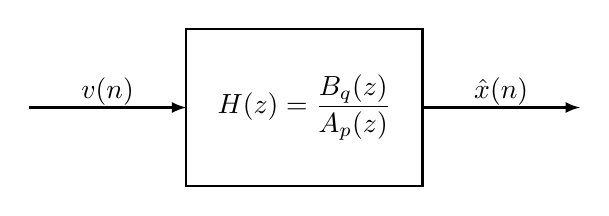
\begin{tikzpicture}
\tikzset{>=latex}
\node at (-1,1.2)  {$v(n)$}; 
\draw[thick,->] (-2,1)--(0,1);
\draw[thick] (0,0) rectangle (3,2) node[pos=.5] {$H(z)=\displaystyle \frac{B_q (z)}{A_p (z)}$};
\draw[thick,->] (3,1)--(5,1);
\node at (4,1.2)  {$\hat{x}(n)$}; 
\end{tikzpicture}
\end{center}
Dieses Modell wird mit einer rationalen Funktion
\begin{equation}
H(z)
=
\frac{B_{q}(z)}{A_{p}(z)}
=
\frac{\displaystyle\sum_{k=0}^{q} b_{q}(k) z^{-k}}{1+\displaystyle\sum_{k=1}^{p} a_{p}(k) z^{-k}}
\end{equation}
beschrieben.
Der Fehler $e^{\prime}$ dieses Modells, ist durch die Differenz des originalen Signales und dem Ausgang des Approximierenden Modells
\begin{equation}
e^{\prime}(n)=x(n)-\hat{x}(n)
\end{equation}
definiert. 
Das Ziel ist es einen Filter $H(z)$ und ein Input $v(n)$, welche $\hat{x}(n)$ so nahe wie möglich an $x(n)$ bringen, zu finden.

Wenn man ein Modell gewählt hat möchte man die besten Parameter oder auch die beste Approximation für sein Modell finden.
Es gibt jedoch sehr viele Arten die beste Approximation zu definieren und damit auch unzählige Methoden um die Modellparameter zu erhalten.
Deshalb ist es wichtig wenn man eine Signalmodellierung angeht eine Methode zu finden welche nicht nur Funktioniert und gute Werte liefert, sondern auch eine Methode zu finden welche effizient berechenbar ist.
Dies ist besonders bei Systemen welche Echtzeit Datenverarbeitung ausschlaggebend.

Um eine solche Approximation zu finden ist die erste Intuition oft den Fehler minimieren zu wollen.
Dies nennt sich auch die Least Squares Methode.
Ziel ist es dabei den quadratischen Fehler 
\begin{equation}
E_{L S}
=
\sum_{n=0}^{\infty}\left|e^{\prime}(n)\right|^{2}
\end{equation}
des Systems zu minimieren.

Aus den Bedienungen der Least Squares Method resultiert eine Menge von nichtlinearen Gleichungen welche möglicherweise sehr schwierig lösbar sind.
Da die Lösungsverfahren welche für die Lösung solcher Gleichungen verwendet wird, wie Newton's method und steepest descent, iterative Methoden sind, sind diese Rechnerisch sehr kostspielig und langsam. 
Aus diesem Grund wird in der Praxis der Ansatz des kleinsten quadratischen Fehlers vermieden. 

Um diese nichtlinearen Gleichungen zu vermeiden und dennoch eine Lösung zu finden, welche uns eine passende Anzahl von $x[n]$ Werten mit der Einheitssprungantwort verbindet, kann ein eleganter Trick, der zur Padé-Approximation führt verwendend werden. 
\begin{equation}
H(z) A_{p}(z)=B_{q}(z)
\end{equation}
In der Zeitebene betrachtet handelt es sich in bei dieser Gleichung um eine Faltung.
\begin{equation}
h(n)+\sum_{k=1}^{p} a_{p}(k) h(n-k)=b_{q}(n)
\end{equation}
Die rechte Seite der Gleichung für $n>q$ ist dabei gleich null.
Die Fallunterscheidung
\begin{equation}
x(n)+\sum_{k=1}^{p} a_{p}(k) x(n-k)
=
\left\{\begin{array}{cc}
b_{q}(n) & 
\quad \text{mit } \quad n=0,1, \ldots, q \\
0 & 
\quad \quad \quad\text{mit } \quad n=q+1, \ldots, q+p
\end{array}\right.
\end{equation}
kann in die Matrixform 
\begin{equation}
\left[\begin{array}{cccc}
x(0) & 0 & \cdots & 0 \\
x(1) & x(0) & \cdots & 0 \\
x(2) & x(1) & \cdots & 0 \\
\vdots & \vdots & & \vdots \\
x(q) & x(q-1) & \cdots & x(q-p) \\
x(q+1) & x(q) & \cdots & x(q-p+1) \\
\vdots & \vdots & & \vdots \\
x(q+p) & x(q+p-1) & \cdots & x(q)
\end{array}\right]
\left[\begin{array}{c}
1 \\
a_{p}(1) \\
a_{p}(2) \\
\vdots \\
a_{p}(p) \\
\end{array}\right]
=
\left[\begin{array}{c}
b_{q}(0) \\
b_{q}(1) \\
b_{q}(2) \\
\vdots \\
b_{q}(q) \\
0 \\
\vdots \\
0
\end{array}\right]
\end{equation}
gebracht werden.
Diese Matrix ist uns schon aus dem Abschnitt \ref{pade:subsection:Pade_erstellen} bekannt. Es handelt sich nämlich um eine Padé-Approximation,
welche wir nun für das Signal mit einer vorgegebener Ordnung berechnen können.

\begin{beispiel}

Die ersten sechs Werte 
\begin{equation*}
\bm x=\left[
\begin{array}{l}
1.0000\\
1.5000\\
0.7500\\
0.3750\\
0.1875 \\
0.0938
\end{array}\right]
\end{equation*}
eines Signales sind vorgegeben.
Das Ziel ist, drei verschiedene Padé-Approximanten mit drei verschiedenen Freiheitsgraden zu finden.
\begin{equation*}\begin{aligned}
&\begin{array}{ll}
\text { All pole } & (q=0, p=2) \\
\text { FIR } & (q=2, p=0)\\
\text { IIR } &(\mathrm{q}=1, \mathrm{p}=1)
\end{array}\\
\end{aligned}\end{equation*}
\begin{enumerate}


\item Das All pole Modell $(q=0,p=2)$ wird in die Matrixform
\begin{equation}\left[\begin{array}{ccc}
x(0) & 0 & 0 \\
x(1) & x(0) & 0 \\
x(2) & x(1) & x(0)
\end{array}\right]\left[\begin{array}{c}
1 \\
a_1 \\
a_2
\end{array}\right]=\left[\begin{array}{c}
b_0 \\
0 \\
0
\end{array}\right]\end{equation}
gebracht. 
Von der ersten Gleichung folgt, dass der Wert $b_0 = x(0)=1$ ergeben muss. 
Weiter können nun die letzten zwei Gleichungen
\begin{equation}\left[\begin{array}{ll}
x(0) & 0 \\
x(1) & x(0)
\end{array}\right]\left[\begin{array}{l}
a_1 \\
a_2
\end{array}\right]=-\left[\begin{array}{l}
x(1) \\
x(2)
\end{array}\right]\end{equation}
eingesetzt und gelöst werden.
\begin{equation}\left[\begin{array}{cc}
1 & 0 \\
1.5 & 1
\end{array}\right]\left[\begin{array}{l}
a_1 \\
a_2
\end{array}\right]=-\left[\begin{array}{c}
1.50 \\
0.75
\end{array}\right]\end{equation}
Die resultierenden Koeffizienten
\begin{equation}
a_1=-1.50 \quad  \quad a_2=1.50
\end{equation}
können nun zusammen mit dem $b0$-Koeffizienten in die Übertragungsfunktion  
Somit erhalten wir als Ergebnis für die Approximation unseres $x(n)$ 
\begin{equation}
H(z)=\frac{1}{1-1.50 z^{-1}+1.50 z^{-2}}.
\end{equation}
Man sollte beachten, dass sich die komplexen Pole nicht im Einheitskreis befinden und somit das Resultat kein stabiles Modell sein wird.
Evaluiert man die Impulsantwort des Systems erhalten wir die folgende Approximation für $x(n)$,
\begin{equation}
\hat{x}=[1,1.500,0.750,-1.125,-2.8125,-2.5312].
\end{equation}
Daraus geht hervor das $x(n)= \hat{x}$ für $n= 0,1,2$ gleich ist, jedoch bei höheren $n$ keine akkurate Approximation liefert.

\item Für das FIR-Modell $(q=2,P=0)$ ist das Resultat einfach mit $A(z)=1$ berechenbar.
Da alle weiteren $a$-Koeffizienten wegfallen werden die $b$-Koeffizienten  mit dem Eingangsignal gleich gesetzt 
\begin{equation}\begin{array}{r}

{\left[\begin{array}{l}
	x(0) \\
	x(1) \\
	x(2)
\end{array}\right]
=
\left[\begin{array}{l}
	b_0 \\
	b_1 \\
	b_2
	\end{array}\right]}
\end{array}\end{equation}.

Somit erhalten wir 
\begin{equation}
H(z)=1+1.50 z^{-1}+0.75 z^{-2}
\end{equation}
als unser Modell.

\item Für das IIR-Modell mit $(q=1,p=1)$ welches die Form
\begin{equation}
H(z)=\frac{b(0)+b(1) z^{-1}}{1+a(1) z^{-1}}
\end{equation}
erhalten wird, sind die Padé-Gleichungen

\begin{equation}\left[\begin{array}{ll}
x(0) & 0 \\
x(1) & x(0) \\
x(2) & x(1)
\end{array}\right]\left[\begin{array}{c}
1 \\
a_1
\end{array}\right]=\left[\begin{array}{c}
b_0 \\
b_1\\
0
\end{array}\right].\end{equation}
Der Pol in der letzten Gleichung 
\begin{equation}
x(2)+a_1 x(1)=0
\end{equation}
kann damit gerechnet werden.
Eingesetzt und nach $a_1$ aufgelöst erhalten wir
\begin{equation}
a_1=-\frac{x(2)}{x(1)}=
-\frac{0.75}{1.5}=
-0.5.
\end{equation}
Mit den bekannten Polen können nun die Nullstellen mit den oberen zwei Gleichungen 
\begin{equation}\left[\begin{array}{c}
b_0 \\
b_1
\end{array}\right]=\left[\begin{array}{cc}
1 & 0 \\
1.5 & 1
\end{array}\right]\left[\begin{array}{c}
1 \\
-0.5
\end{array}\right]=\left[\begin{array}{l}
1 \\
1
\end{array}\right]\end{equation}
berechnet werden.
Die Koeffizienten können nun in das Modell eingesetzt werden, womit wir
\begin{equation}
H(z)=\frac{1+z^{-1}}{1-0.5 z^{-1}}
\end{equation}
erhalten.
Dieses Modell hat eine identische Impulsantwort 
\begin{equation}
h(n)=(0.5)^{n} u(n)+(0.5)^{n-1} u(n-1)
=
\delta(n)+1.5(0.5)^{n-1} u(n-1)\end{equation}
wie $x(n)$.
Erkennbar wenn man $n=0$ bis $n=5$ in $h(n)$ einsetzt.
\begin{align*}
h(0)&=\delta(0)+1.5(0.5)^{0-1} u(0-1)=1\\
h(1)&=\delta(1)+1.5(0.5)^{1-1} u(1-1)=1.5\\
h(2)&=\delta(2)+1.5(0.5)^{2-1} u(2-1)=0.75\\
h(3)&=\delta(3)+1.5(0.5)^{3-1} u(3-1)=0.375\\
h(4)&=\delta(4)+1.5(0.5)^{4-1} u(4-1)=0.1875\\
h(5)&=\delta(5)+1.5(0.5)^{5-1} u(5-1)=0.09375\\
\end{align*}
Im Vergleich noch einmal $\bm x$ welches Padé-Approximiert wurde
\begin{equation*}
\bm x=[1.0000 , 1.5000, 0.7500 , 0.3750 , 0.1875, 0.0938]^{T}.
\end{equation*}
Dies ist jedoch ein Spezialfall und kommt nicht immer vor.
\end{enumerate}
\end{beispiel}






